%%%%%%%%%%%%%%%%%%%%%%%%%%%%%%%%%%%%%%%%%
% a0poster Portrait Poster
% LaTeX Template
% Version 1.0 (22/06/13)
%
% The a0poster class was created by:
% Gerlinde Kettl and Matthias Weiser (tex@kettl.de)
% 
% This template has been downloaded from:
% http://www.LaTeXTemplates.com
%
% License:
% CC BY-NC-SA 3.0 (http://creativecommons.org/licenses/by-nc-sa/3.0/)
%
%%%%%%%%%%%%%%%%%%%%%%%%%%%%%%%%%%%%%%%%%

%----------------------------------------------------------------------------------------
%	PACKAGES AND OTHER DOCUMENT CONFIGURATIONS
%----------------------------------------------------------------------------------------

\documentclass[a0,portrait]{a0poster}

\usepackage{multicol} % This is so we can have multiple columns of text side-by-side
\columnsep=100pt % This is the amount of white space between the columns in the poster
\columnseprule=3pt % This is the thickness of the black line between the columns in the poster

\usepackage[svgnames]{xcolor} % Specify colors by their 'svgnames', for a full list of all colors available see here: http://www.latextemplates.com/svgnames-colors

\usepackage{times} % Use the times font
%\usepackage{palatino} % Uncomment to use the Palatino font
\usepackage{subcaption}
\usepackage{amsmath,amsfonts,amssymb,amsthm,mathtools}
\usepackage{indentfirst}
\usepackage{minted}
\usepackage{verbatim}
\usepackage{graphics}
\usepackage{float}
\usepackage{multicol}
\usepackage{titlesec}
\usepackage{graphicx} % Required for including images
\graphicspath{{figures/}} % Location of the graphics files
\usepackage{booktabs} % Top and bottom rules for table
\usepackage[font=small,labelfont=bf]{caption} % Required for specifying captions to tables and figures
\usepackage{amsfonts, amsmath, amsthm, amssymb} % For math fonts, symbols and environments
\usepackage{wrapfig} % Allows wrapping text around tables and figures

\setlength{\parindent}{1em}
\setlength{\parskip}{0pt}



\begin{document}

%----------------------------------------------------------------------------------------
%	POSTER HEADER 
%----------------------------------------------------------------------------------------

% The header is divided into two boxes:
% The first is 75% wide and houses the title, subtitle, names, university/organization and contact information
% The second is 25% wide and houses a logo for your university/organization or a photo of you
% The widths of these boxes can be easily edited to accommodate your content as you see fit

\begin{minipage}[b]{0.85\linewidth}
\veryHuge \color{NavyBlue} \textbf{1D-to-3D crossover on multileg attractive-U Hubbard ladders} \color{Black}\\[2cm] % Title
%\Huge\textit{An Exploration of Complexity}\\[2cm] % Subtitle
\huge \textbf{Anastasia Potapova, Ian Pile, Evgeni Burovski}\\[0.5cm] % Author(s)
\huge HSE University, Moscow, Russia\\[0.4cm] % University/organization
\Large \texttt{anastaciya.potapova@gmail.com}\\
\end{minipage}
%
\vspace{0.8cm} % A bit of extra whitespace between the header and poster content

%----------------------------------------------------------------------------------------

\begin{multicols}{2} % This is how many columns your poster will be broken into, a portrait poster is generally split into 2 columns

%----------------------------------------------------------------------------------------
%	ABSTRACT
%----------------------------------------------------------------------------------------

\color{Navy} % Navy color for the abstract

\begin{abstract}

We study ground state properties of a polarized two-component Fermi gas on  multileg attractive-U Hubbard ladders. Using DMRG simulations, we construct  grand canonical phase diagrams for varying perpendicular geometries and  ratios of hopping amplitudes, and characterize the 1D-to-3D crossover.  We compare our findings with recent experimental and theoretical studies of  quasi-one-dimensional polarized Fermi gases.

\end{abstract}

%----------------------------------------------------------------------------------------
%	INTRODUCTION
%----------------------------------------------------------------------------------------


%----------------------------------------------------------------------------------------
%	OBJECTIVES
%----------------------------------------------------------------------------------------

\color{DarkSlateGray} % DarkSlateGray color for the rest of the content


%----------------------------------------------------------------------------------------
%	MATERIALS AND METHODS
%----------------------------------------------------------------------------------------

\section*{Model and Methods}

We consider the attractive-U Hubbard model of a two-component Fermi gas at zero temperature on a $W \times L$ ladder defined by the Hamiltonian,

\begin{equation} \label{Hubbard}
\hat{H}=-t \sum_{i} \left( \hat{c}_{i,\sigma}^{\dagger} \hat{c}_{i+1, \sigma} + h.c. \right) - U \sum_{i} \hat{n}_{i, \uparrow} \hat{n}_{i, \downarrow}
\end{equation}

where $t$ is the hopping amplitude, $\hat{c}_{i,\sigma}^{\dagger}$ is the creation operator for a fermion with spin $\sigma$ at site $i$, $\hat{c}_{i,\sigma}$ is the annihilation operator for a fermion. The summation in the equation \eqref{Hubbard} runs over $L \dot W$ sites, where $L$ is the length of a $W$-leg ladder. $U$ is the interaction parameter between two fermions with the opposite spins on site, $\hat{n}_{i, \sigma}$ is the number of particles operator with spin $\sigma = \downarrow, \uparrow$.

\begin{center}\vspace{0.9cm}
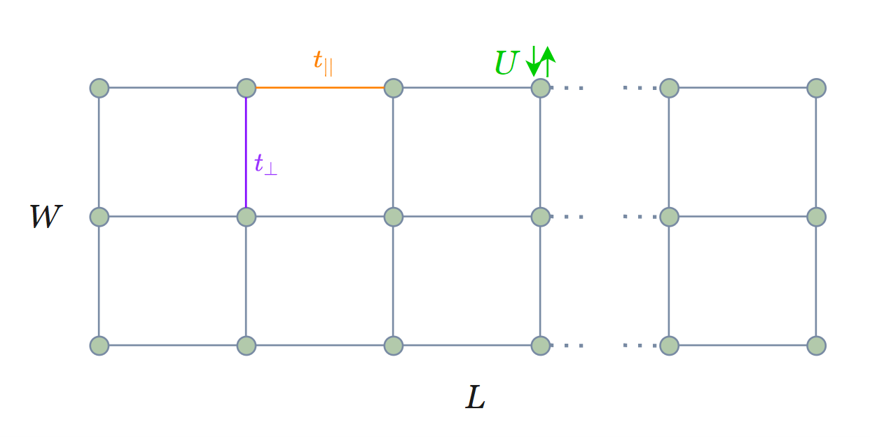
\includegraphics[width=0.5\linewidth]{lattice.png}
\captionof{figure}{Schematic of the 3-leg ladder lattice. }
\end{center}\vspace{0.9cm}

We compute the ground state energies $E(N_{\uparrow}, N_{\downarrow})$ of the model \eqref{Hubbard} using density matrix renormalization group (DMRG) simulations. Here $N_{\uparrow}$ is the number of spin-up particles, $N_{\downarrow}$ is the number of spin-down particles.

Ground state energies are needed to construct a phase diagram of a system. The variables of a phase diagram are the effective magnetic field $h$ and the chemical potential $\mu$:

\begin{equation} \label{mu}
\mu = {\left( \frac{\partial E}{\partial N_{+}} \right)}_{N_{-}}
\end{equation}
	
\begin{equation} \label{h}
h = {\left( \frac{\partial E}{\partial N_{-}} \right)}_{N_{+}}
\end{equation}
	 
where $N_{+} = N_{\uparrow} + N_{\downarrow}$ and $N_{-} = N_{\uparrow} - N_{\downarrow}$.

Phases that we are interested in:

\begin{enumerate} 
    \item Vacuum ($V$): $N_{\uparrow} = N_{\downarrow} = 0$
    \item Equal Densities ($ED$): $N_{\uparrow} = N_{\downarrow}$
    \item Partially polarized ($PP$): $N_{\uparrow} > N_{\downarrow}$
    \item Fully polarized 1 ($FP_1$): $0 < N_{\uparrow} < L \times W,  N_{\downarrow} = 0$
    \item Fully polarized 2 ($FP_2$): $N_{\uparrow} = W\times L,  N_{\downarrow} = 0$
\end{enumerate}

We approximate the derivatives \eqref{mu}, \eqref{h} with finite differences and getting the following equations for each phase:

\begin{enumerate}
\item The boundary between $ED$ and $PP$ ($ED-PP$)

\begin{equation} \label{ED-PP mu}
\mu = {\left( \frac{\partial E}{\partial N_{+}} \right)}_{N_{-}} = \frac{E(N_{\uparrow} + 1, N_{\downarrow} + 1) - E(N_{\uparrow} ,N_{\downarrow})}{2}
\end{equation}
	
\begin{equation}\label{ED-PP h}
h = {\left( \frac{\partial E}{\partial N_{-}} \right)}_{N_{+}} = \frac{E(N_{\uparrow} + 1, N_{\downarrow} - 1) - E(N_{\uparrow} ,N_{\downarrow})}{2}
\end{equation}

\item The boundary between $PP$ and $FP_1$

\begin{equation} \label{PP-FP1 mu}
\mu = {\left( \frac{\partial E}{\partial N_{+}} \right)}_{N_{-}} = \frac{E(N_{\uparrow} + 1, 1) - E(N_{\uparrow}, 0)}{2}
\end{equation}

\begin{equation} \label{PP-FP2 h}     	
h = {\left( \frac{\partial E}{\partial N_{-}} \right)}_{N_{+}} = \frac{E(N_{\uparrow} - 1, 1) - E(N_{\uparrow}, 0)}{-2}
\end{equation}

\item The boundary between $ED$ and $V$
\begin{equation}
\mu = \frac{E(1, 1)}{2}
\end{equation}
     	
\item The boundary between $V$ and $FP_1$
\begin{equation} \label{V-FP}
\mu = - h + E(1, 0)
\end{equation}
     	
\item The boundary between $FP_1$ and $FP_2$

\begin{equation} \label{FP-FP}
\mu = - h - E(1, 0)
\end{equation}

\end{enumerate}
     
%------------------------------------------------



%----------------------------------------------------------------------------------------
%	RESULTS 
%----------------------------------------------------------------------------------------

\section*{Results}
  

We construct phase diagrams for quasi-one dimensional multileg ladders, using equations \eqref{PP-FP1 mu}-\eqref{FP-FP}. The boundaries of the phase diagrams are parameterized by $N_{\uparrow}$/.

The grand canonical phase diagram of a one-dimensional chain is displayed in Fig. 1 (a) For two- and three-leg ladders there are Fig 1.(b) and Fig.1 (c). Diagrams are constructed for $U = -7, t = 1, L = 40$.

%\begin{center}\vspace{1cm}
%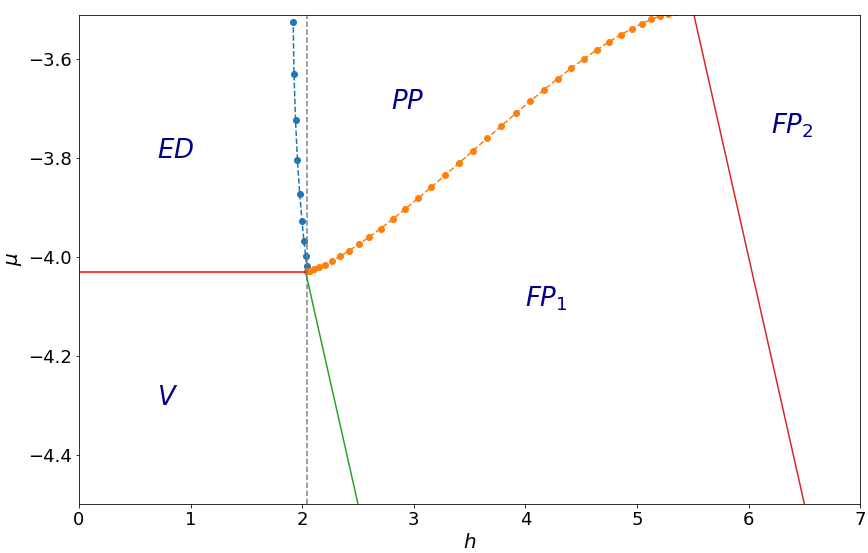
\includegraphics[width=0.8\linewidth]{w1.png}
%\captionof{figure}{\color{Green} The phase diagram for $W = 1$}
%\end{center}\vspace{1cm}

%\begin{center}\vspace{1cm}
%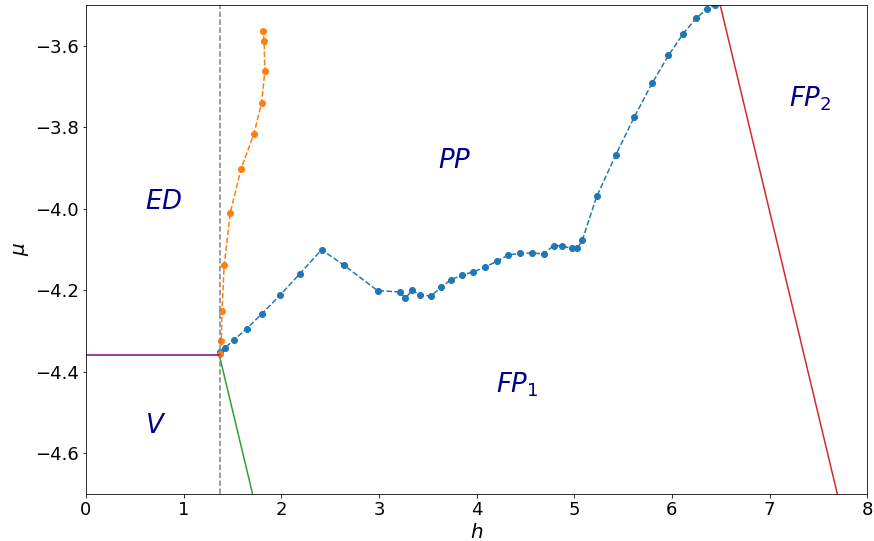
\includegraphics[width=0.8\linewidth]{w2.png}
%\captionof{figure}{\color{Green} The phase diagram for $W = 2$}
%\end{center}\vspace{1cm}

%\begin{center}\vspace{1cm}
%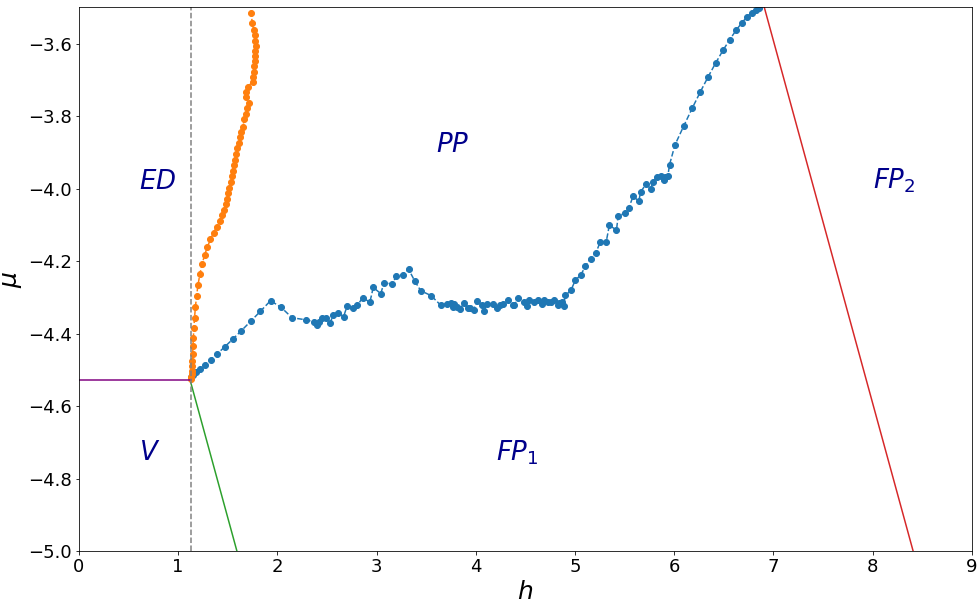
\includegraphics[width=0.8\linewidth]{w=3.png}
%\captionof{figure}{\color{Green} The phase diagram for $W = 3$}
%\end{center}\vspace{1cm}

\begin{figure}[H]
    \centering
    \begin{subfigure}[t]{0.23\textwidth}
        %\begin{tikzpicture}
        \centering
        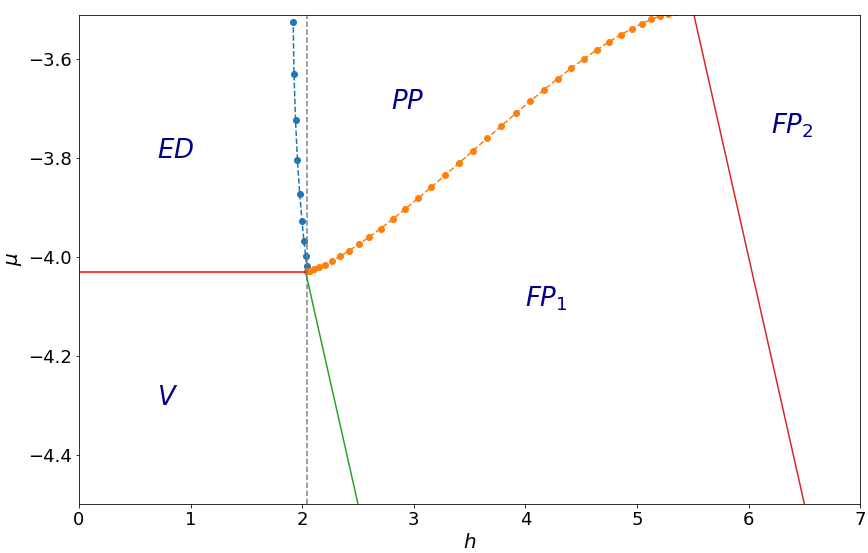
\includegraphics[width=\linewidth]{w1.png}
        \caption{}
        %\end{tikzpicture}   
    \end{subfigure}
    \hfill
    \begin{subfigure}[t]{0.23\textwidth}
        %\begin{tikzpicture}
        \centering
        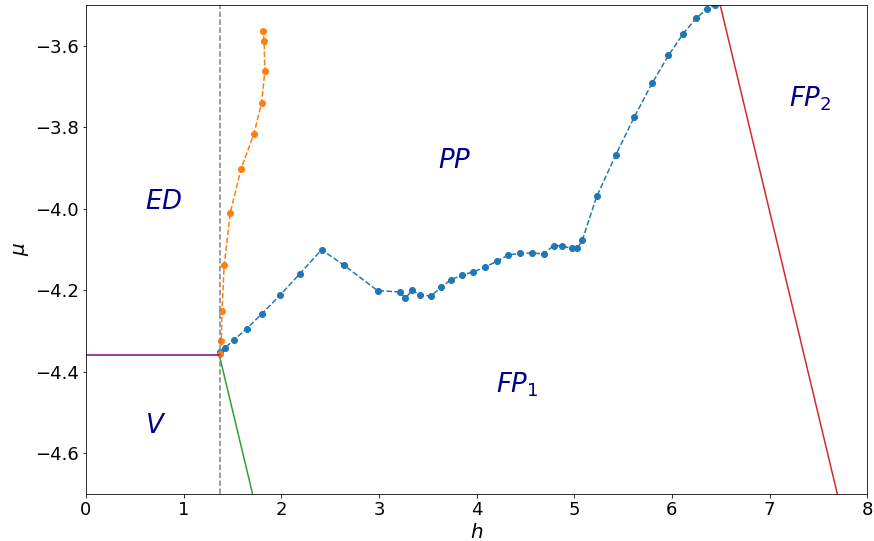
\includegraphics[width=\linewidth]{w2.png}
        \caption{}
        %\end{tikzpicture}
     \end{subfigure}

    \centering
    \begin{subfigure}[t]{0.23\textwidth}
        %\begin{tikzpicture}
        \centering
        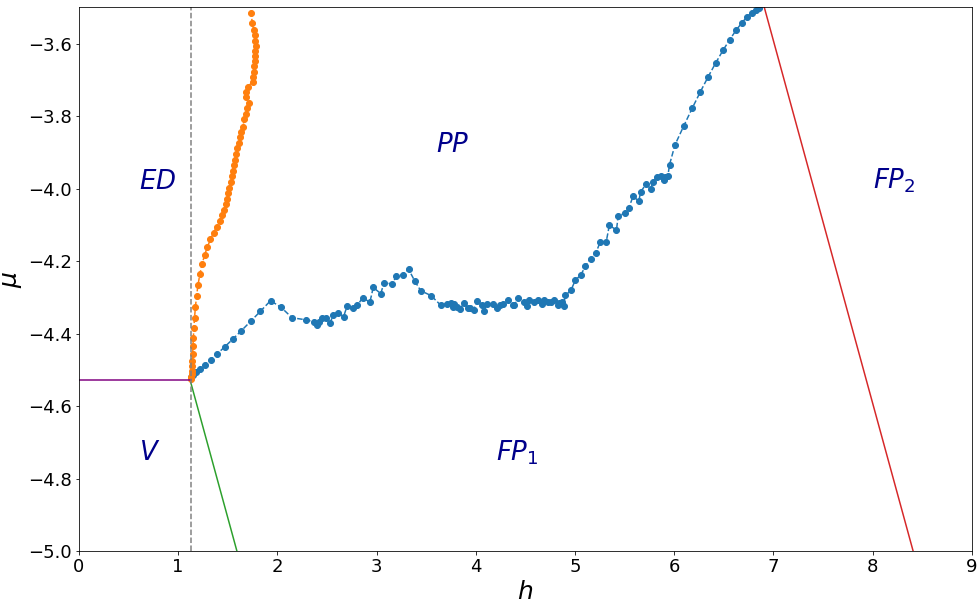
\includegraphics[width=\linewidth]{w=3.png}
        \caption*{(c)}
        %\end{tikzpicture}   
    \end{subfigure}
    \hfill
    \begin{subfigure}[t]{0.23\textwidth}
        %\begin{tikzpicture}
        \centering
        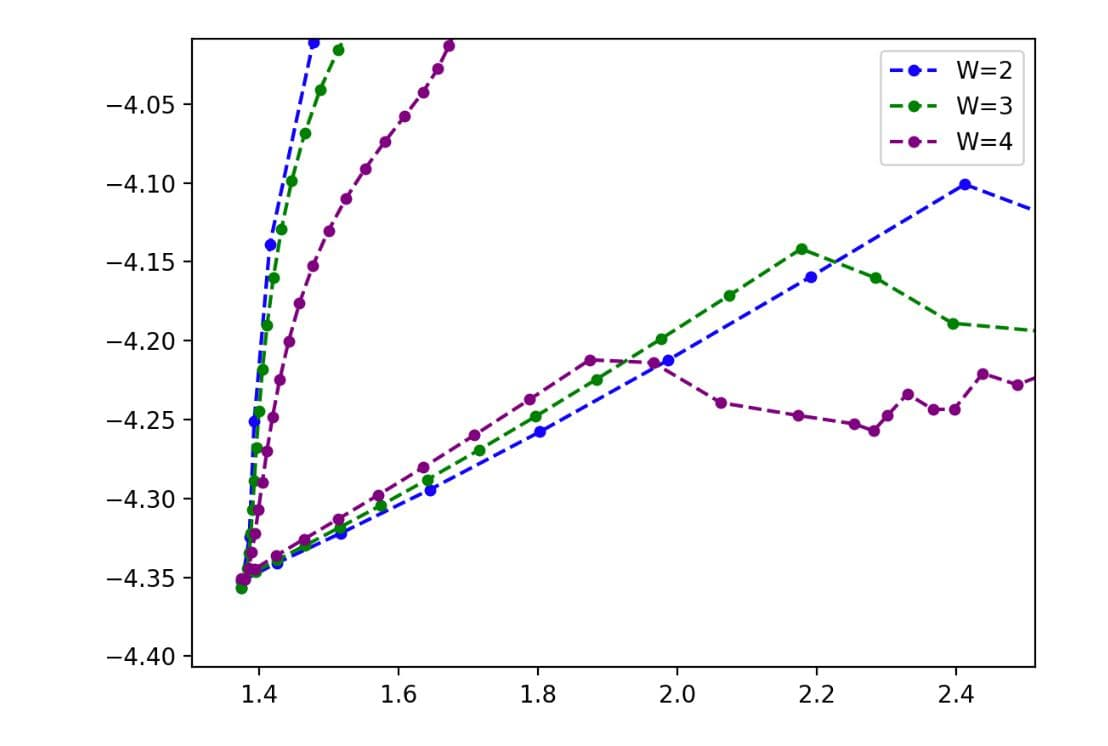
\includegraphics[width=\linewidth]{copm234.jpg}
        \caption*{(d)}
        %\end{tikzpicture}
     \end{subfigure}
     \caption{The phase diagrams for  (a) $W = 1$, (b) $W = 2$, (c) $W = 3$, (d) the vicinity of the multicritical point $W = 2, 3, 4$}
\label{pol}
\end{figure}


%----------------------------------------------------------------------------------------
%	CONCLUSIONS
%----------------------------------------------------------------------------------------
As shown in Fig.2 (a) - (c) the phase diagram of a one-dimensional system differs qualitatively from the phase diagram of 2-3-leg ladders. The main and important difference is the boundary between the equal density phase and the partially polarized phase ($ED-PP$ in Fig.2), since the phase diagram characterizes the structure of the atomic cloud shell in experiments with ultra cold Fermi gases. In 1D case $\frac{\partial \mu}{\partial h} < 0$, while for two and three leg ladders $\frac{\partial \mu}{\partial h} > 0$. Our results is consistent with recent experimental papers \cite{liao}-\cite{shin}. In particular, Ref. \cite{revelle} characterizes the 1D-3D dimensional crossover of a two-component spin polarized Fermi gas of $ ^{6}$Li in a 2D optical lattice by varying the lattice depth and interactions. 

In 1D system at some value of polarization in an atomic cloud the $PP$ phase is located in the centre of the cloud and the $ED$ phase occupies the wings of the atomic cloud. The $ED$ phase absents if the polarization goes larger. The relative location of these phases in 3D is inverted compared to 1D. The $ED$ phase core is surrounded by the $PP$ phase. The fully polarized phase $FP$ is located outside the $PP$ phase. 

By setting values of the effective magnetic field $h$ and varying the chemical potential $\mu$, we can obtain from the phase diagrams in Fig. 2 (a)-(c) exactly the same phase structure of the atomic cloud as it has previously described.

The one more difference between 1-leg and 2- and 3-leg ladder systems is that the boundary between partially polarized and fully polarized phases is non-monotonic. This can be due to the filling of energy bands in the spectrum. The non-monotonic area in phase diagrams corresponds to energies of a non-interacting system that is in the intersection of two (or three in 3-leg ladder) energy bands.

Our results for 1-leg ladder agree with \cite{oneleg ladder} and \cite{burovski}, for 2-leg ladder results agree with DMRG computing of Ref.\cite{twoleg ladder}

\section*{Ongoing Research}

We are computing phase diagram for 2-3-4 leg ladders using DMRG and varying the transverse hopping amplitude $t_{\perp}$ for each system. %We're comparing our results with Ref.
Current result is depicted in Fig. 3. It shows the phase diagram evolution of the 2-leg ladder system (a) and the evolution of $ED-PP$ boundary with varying $t_{\perp}$ (b). 

\begin{figure}[H]
    \centering
    \begin{subfigure}[t]{0.23\textwidth}
        %\begin{tikzpicture}
        \centering
        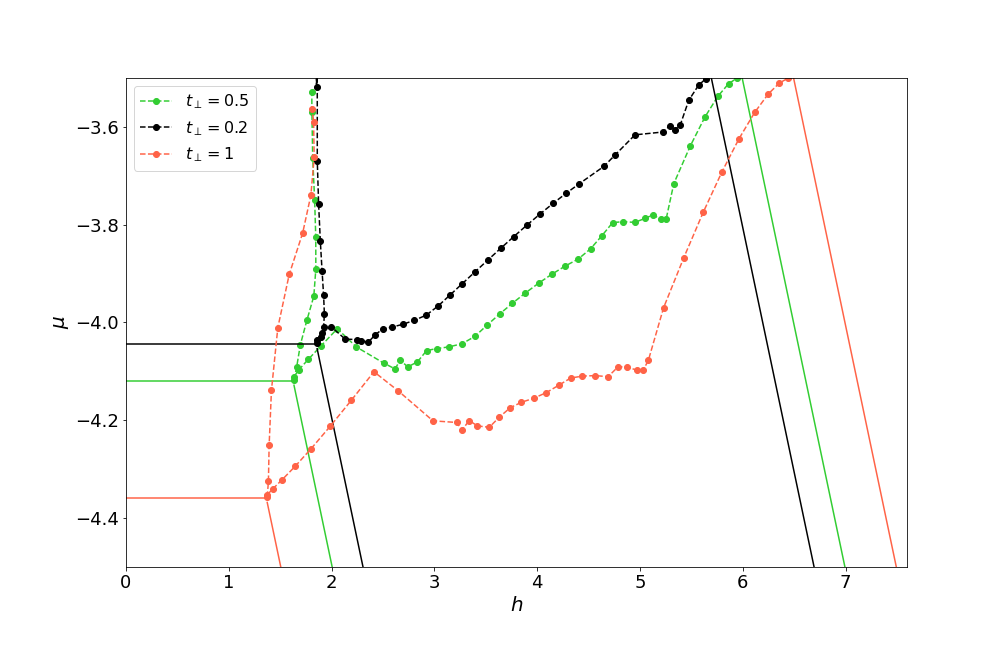
\includegraphics[width=\linewidth]{tperp.png}
        \caption{}
        %\end{tikzpicture}   
    \end{subfigure}
    \hfill
    \begin{subfigure}[t]{0.23\textwidth}
        %\begin{tikzpicture}
        \centering
        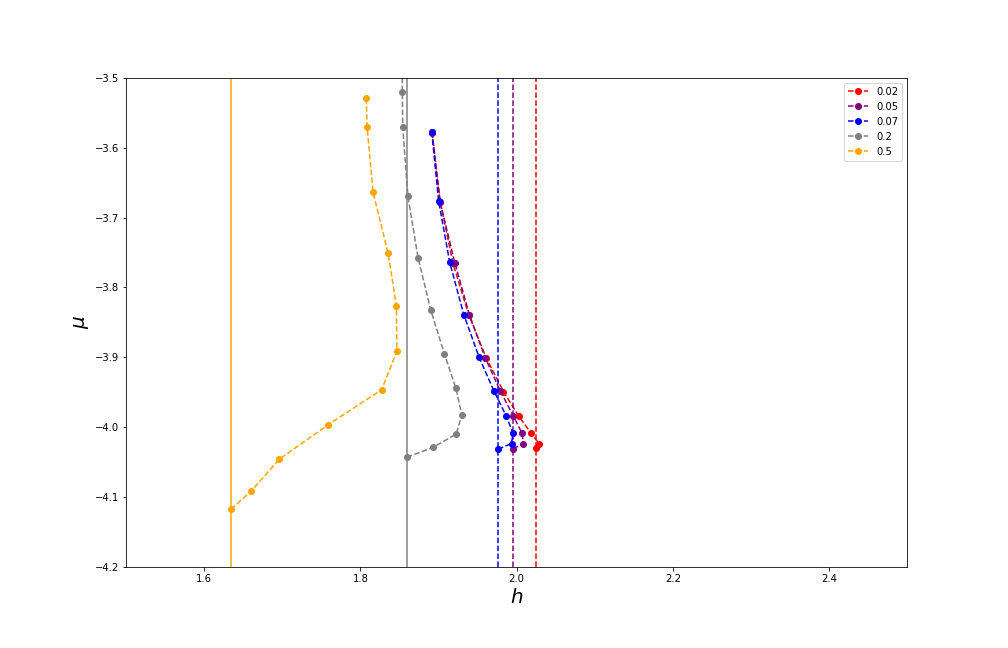
\includegraphics[width=\linewidth]{comparison_ED-PP_tperp.png}
        \caption{}
        %\end{tikzpicture}
     \end{subfigure}
     \caption{(a) The phase diagram evolution for $W = 2$ with varying $t_{\perp}$. Black line $t_{\perp} = 0.2$, green line $t_{\perp} = 0.5$, orange line $t_{\perp} = 1$ (b) The evolution of ED-PP boundary with varying $t_{\perp}$. Yellow line $t_{\perp} = 0.5$, grey line $t_{\perp} = 0.2$, blue, purple and red lines $t_{\perp} = 0.07, 0.05, 0.02$ respectively.}
\end{figure}

 %----------------------------------------------------------------------------------------
%	REFERENCES
%----------------------------------------------------------------------------------------

%\nocite{*} % Print all references regardless of whether they were cited in the poster or not
%\bibliographystyle{plain} % Plain referencing style
%\bibliography{sample} % Use the example bibliography file sample.bib
\begin{thebibliography}{}

\bibitem{liao}Liao Y, Rittner A S C, Paprotta T \textit{et al}, \textit{Nature}, \textbf{467}, 567–569 (2010)

\bibitem{revelle}Revelle M C, Fry J A, Olsen B A and Hulet R G, \textit{Phys. Rev. Lett.} \textbf{117} 235301 (2016)

\bibitem{shin}Shin Y, Zwierlein M W, Schunck C Y, \textit{Phys. Rev. Lett.}  \textbf{97} 030401 (2006)

\bibitem{oneleg ladder} F. Heidrich-Meisner, G. Orso, and A. E. Feiguin
\textit{Phys. Rev. A} \textbf{81}, 053602 (2010) 

\bibitem{twoleg ladder} A. E. Feiguin and F. Heidrich-Meisnerm \textit{Phys. Rev. Lett.} \textbf{102}, 076403 (2009) 

\bibitem{burovski}E.A. Burovski, R.Sh. Ikhsanov, A.A. Kuznetsov and M.Yu. Kagan, \textit{J. Phys.: Conf. Ser} \textbf{1163} 012046 (2019) 

\end{thebibliography}

\end{multicols}
\end{document}